% !TEX encoding = UTF-8
% !TEX root = experiment_report.tex
% 慧眼——智能垃圾分类与回收建议系统 实验报告
%
% 编译方法（两次编译）:
%   xelatex experiment_report.tex
%   xelatex experiment_report.tex
%
\documentclass[11pt,a4paper]{ctexart}

% ============ Packages ============
\usepackage[top=0.8in, bottom=0.8in, left=0.9in, right=0.9in]{geometry}
\usepackage{graphicx}
\usepackage{amsmath,amssymb}
\usepackage{booktabs}
\usepackage{tabularx}
\usepackage{xcolor}
\usepackage{listings}
\usepackage{hyperref}
\usepackage{fancyhdr}
\usepackage{caption}
\usepackage{float}
\usepackage{enumitem}

% ============ Compact spacing ============
\setlength{\parskip}{2pt plus 1pt}
\setlength{\parindent}{1.5em}
\setlength{\abovecaptionskip}{4pt}
\setlength{\belowcaptionskip}{2pt}
\setlength{\intextsep}{4pt plus 1pt}
\setlength{\textfloatsep}{6pt plus 1pt}
\setlength{\floatsep}{4pt plus 1pt}
\setlength{\abovedisplayskip}{4pt plus 1pt}
\setlength{\belowdisplayskip}{4pt plus 1pt}
\setlength{\abovedisplayshortskip}{2pt plus 1pt}
\setlength{\belowdisplayshortskip}{2pt plus 1pt}
\linespread{1.08}
\usepackage{etoolbox}
\AtBeginEnvironment{table}{\vspace{-4pt}}
\AtEndEnvironment{table}{\vspace{-4pt}}
\AtBeginEnvironment{figure}{\vspace{-4pt}}
\AtEndEnvironment{figure}{\vspace{-4pt}}
\setlist{nosep,left=2em,topsep=1pt,partopsep=0pt}
% Tighten section spacing
\usepackage{titlesec}
\titlespacing{\section}{0pt}{8pt}{4pt}
\titlespacing{\subsection}{0pt}{6pt}{2pt}
\titlespacing{\subsubsection}{0pt}{4pt}{2pt}

% ============ Hyperref ============
\hypersetup{
  colorlinks=true,
  linkcolor=black,
  urlcolor=blue,
  citecolor=black,
}

% ============ Header/Footer ============
\pagestyle{fancy}
\fancyhf{}
\fancyhead[C]{慧眼——智能垃圾分类与回收建议系统 · 实验报告}
\fancyfoot[C]{—\ \thepage\ —}
\renewcommand{\headrulewidth}{0.4pt}

% ============ Code Style ============
\definecolor{codebg}{RGB}{245,245,245}
\lstset{
  backgroundcolor=\color{codebg},
  basicstyle=\ttfamily\small,
  breaklines=true,
  frame=none,
  columns=flexible,
  keepspaces=true,
  showstringspaces=false,
  aboveskip=4pt,
  belowskip=4pt,
  xleftmargin=20pt,
}

% ============ New Commands ============
\newcommand{\rb}[1]{\ensuremath{\mathbb{R}^{#1}}}
\newcommand{\figref}[1]{图\ref{#1}}
\newcommand{\tabref}[1]{表\ref{#1}}

% ============ Title Page Info ============
\title{}
\author{}
\date{}

\begin{document}

% ==================== COVER ====================
\begin{titlepage}
\centering
\vspace*{2cm}
{\heiti\fontsize{32pt}{40pt}\selectfont 实验报告\par}
\vspace{1cm}
{\heiti\fontsize{26pt}{34pt}\selectfont\color[HTML]{2E7D32} 慧眼——智能垃圾分类与回收建议系统\par}
\vspace{0.8cm}
{\songti\fontsize{14pt}{20pt}\selectfont\color[HTML]{666666} 基于 PyTorch 的 ResNet18 多任务垃圾分类模型\par}
\vspace{2cm}
{\songti\fontsize{14pt}{20pt}\selectfont\color[HTML]{888888} 2026 年 6 月\par}
\end{titlepage}

\fancyhead[C]{慧眼——智能垃圾分类与回收建议系统 · 实验报告}

% ==================== CHAPTER 1 ====================
\section{核心原理与算法设计}

\subsection{问题定义}

垃圾分类是典型的多分类问题。给定输入图像 $x \in \rb{3 \times H \times W}$，模型需要输出类别概率分布 $\hat{y} \in \rb{10}$（电池、厨余、纸板、衣物、玻璃、金属、纸张、塑料、鞋子、其他），以及四个二分类属性预测（is\_bottle: 是否瓶子、liquid: 有无液体、flatten: 是否压扁、spread: 是否展平）。模型采用共享骨干 + 多分支头的架构。

\subsection{CNN 骨干网络}

\subsubsection{自建 CNN 骨干（3×ConvBlock）}

自建 CNN 骨干网络由三个卷积块（ConvBlock）堆叠而成。每个 ConvBlock 包含四个子层：
\[
\text{Conv2d} \rightarrow \text{BatchNorm2d} \rightarrow \text{ReLU} \rightarrow \text{MaxPool2d}
\]
这种经典设计遵循 CNN 层级特征提取范式——浅层卷积捕获边缘和纹理等低级特征，深层卷积组合出具有类别判别性的高级语义特征。

三个 ConvBlock 的通道数配置为 $[3\rightarrow64,\; 64\rightarrow128,\; 128\rightarrow256]$。由于每个 MaxPool2d 的池化核大小均为 $2\times2$、步长也为 $2$，经过三层后特征图的空间尺寸缩小为原始输入的 $1/8$。

\vspace{4pt}
\textbf{自建 CNN 完整的 Matrix Shape 变换过程如下：}
\begin{lstlisting}
Input:          [B, 3,   224, 224]
ConvBlock1:     [B, 64,  112, 112]    // 3->64 ch, MaxPool down
ConvBlock2:     [B, 128, 56,  56 ]    // 64->128 ch, MaxPool down
ConvBlock3:     [B, 256, 28,  28 ]    // 128->256 ch, MaxPool down
GlobalAvgPool:  [B, 256, 1,   1  ]    // AdaptiveAvgPool2d(1)
Flatten:        [B, 256]
Dropout(0.5):   [B, 256]
FC + ReLU:      [B, 512]
Classifier:     [B, 10]               // main class head
Task Heads:     [B, 2] x 4            // 4 attr branch
\end{lstlisting}

\subsubsection{ResNet18 骨干（预训练）}

当 backbone 参数设为 \texttt{"resnet18"} 时，模型使用 torchvision 中的 ResNet18 作为骨干网络。去掉原始 ResNet18 最后的全连接分类层（保留到 layer4 的最后一个 conv2 层），输出 512 维特征向量。ResNet18 的通过在卷积块输入和输出之间建立恒等映射（残差连接），有效缓解了深层网络的梯度消失问题，使得模型能够更好地利用 ImageNet 预训练权重中蕴含的通用视觉知识进行迁移学习。

\vspace{4pt}
\textbf{ResNet18 骨干的 Matrix Shape 变换过程：}
\begin{lstlisting}
Input:           [B, 3,   224, 224]
conv1+bn1+relu:  [B, 64,  112, 112]
maxpool:         [B, 64,  56,  56 ]
layer1 (2 blocks): [B, 64,  56,  56 ]    // ch fixed
layer2 (2 blocks): [B, 128, 28,  28 ]    // ch 2x, /2 spatial
layer3 (2 blocks): [B, 256, 14,  14 ]    // ch 2x, /2 spatial
layer4 (2 blocks): [B, 512, 7,   7  ]    // ch 2x, /2 spatial
avgpool:         [B, 512, 1,   1  ]    // AdaptiveAvgPool2d
Flatten:         [B, 512]
Dropout(0.5):    [B, 512]
FC + ReLU:       [B, 512]
Classifier:      [B, 10]
Task Heads:      [B, 2] x 4
\end{lstlisting}

\subsection{前向传播与 Matrix Shape 变换的数学推导}

\subsubsection{卷积层前向传播}

对于二维卷积层，给定输入张量 $X \in \rb{B \times C_{in} \times H_{in} \times W_{in}}$，卷积核（滤波器）$W \in \rb{C_{out} \times C_{in} \times K \times K}$，偏置 $b \in \rb{C_{out}}$（本项目模型因后续接 BatchNorm 层，故卷积层设置 bias=False）。输出特征图 $Y \in \rb{B \times C_{out} \times H_{out} \times W_{out}}$ 的计算公式为：
\begin{equation}
Y[b, c_{out}, i, j] = \sum_{c_{in}} \sum_{u} \sum_{v} X[b, c_{in}, i+u, j+v] \cdot W[c_{out}, c_{in}, u, v]
\end{equation}

本模型中 padding 设为 $K/2$（即 kernel\_size=3 时 padding=1），stride=1，因此卷积操作不改变空间尺寸。下采样由 MaxPool2d(2,2) 完成：
\begin{equation}
H_{out} = \lceil H_{in} / 2 \rceil,\quad W_{out} = \lceil W_{in} / 2 \rceil
\end{equation}

\subsubsection{BatchNorm 层}

Batch Normalization 对每个通道独立进行归一化。设小批量 $\mathcal{B}$ 在第 $c$ 个通道上的均值为 $\mu_c$、方差为 $\sigma_c^2$，可学习参数为 $\gamma_c$（缩放因子）和 $\beta_c$（平移因子）：
\begin{align}
\hat{x}_c &= \frac{x_c - \mu_c}{\sqrt{\sigma_c^2 + \varepsilon}} \\
y_c &= \gamma_c \cdot \hat{x}_c + \beta_c
\end{align}
其中 $\varepsilon = 10^{-5}$ 为防止除零的小常数。BatchNorm 通过减少内部协变量偏移（Internal Covariate Shift）加速收敛，同时起到轻微的正则化效果。

\subsubsection{全连接层与激活函数}

经过 Global Average Pooling 和 Flatten 操作后，特征向量 $z \in \rb{B \times D}$ 进入全连接层（其中 $D=256$ 对应自建 CNN 骨干，$D=512$ 对应 ResNet18 骨干）。全连接层执行线性变换：
\begin{equation}
h = W_{fc} \cdot z + b_{fc},\qquad W_{fc} \in \rb{512 \times D},\; z \in \rb{B \times D}
\end{equation}

随后通过 ReLU（Rectified Linear Unit）激活函数引入非线性：
\begin{equation}
a = \max(0, h)
\end{equation}

最后的分类头将 512 维特征映射为各类别的 logits：
\begin{align}
\text{logits}_{cls} &= W_{cls} \cdot a + b_{cls}, \qquad W_{cls} \in \rb{10 \times 512} \\
\text{logits}_{task_k} &= W_{task_k} \cdot a + b_{task_k}, \quad W_{task_k} \in \rb{2 \times 512}
\end{align}
其中 $k \in \{\text{is\_bottle}, \text{liquid}, \text{flatten}, \text{spread}\}$，分别对应四个属性检测任务。

\subsection{损失函数设计}

\subsubsection{Focal Loss（焦点损失）}

垃圾分类数据集中各类别样本数量存在显著不平衡（如「纸张」类别样本较少）。为缓解这一问题，本模型采用 Focal Loss 替代标准交叉熵损失。Focal Loss 由 Lin 等人于 2017 年在 RetinaNet 论文中提出，其核心思想是通过引入调制因子 $(1-p_t)^\gamma$ 降低易分类样本的损失权重，使训练过程聚焦于难分类样本。

标准交叉熵损失的表达式为：
\begin{equation}
\mathrm{CE}(p_t) = -\log(p_t)
\end{equation}
其中 $p_t$ 为模型对真实类别的预测概率。Focal Loss 在此基础上进行修正：
\begin{equation}
\mathrm{FL}(p_t) = -\alpha_t \cdot (1-p_t)^\gamma \cdot \log(p_t)
\end{equation}

参数说明：(1) $\alpha_t$——类别权重因子。本模型通过统计训练集中各类别样本数量自动计算，公式为 $\alpha_i = N_{total} / (10 \times N_i)$。此外还支持 class\_boost 参数对特定少数类手动提升权重（默认对 paper 施加 $1.5\times$、glass 施加 $1.3\times$ 的补偿），使模型给予这些类别更多关注；(2) $\gamma$——聚焦参数（默认 $\gamma = 2.0$）。当 $\gamma = 0$ 时 Focal Loss 退化为加权交叉熵；$\gamma$ 越大，易分样本（$p_t \to 1$）的损失贡献被压制得越强。

直观示例：当模型对某样本的预测概率 $p_t = 0.9$（易分样本）且 $\gamma = 2$ 时，$(1-0.9)^2 = 0.01$，该样本的损失被压缩为原来的 $1\%$；而当 $p_t = 0.1$（难分样本）时，$(1-0.1)^2 = 0.81$，损失几乎不变。因此，模型在训练过程中自然地将更多注意力分配给难以正确分类的样本。

\subsubsection{多任务联合损失}

在多任务学习模式下，总损失函数定义为主分类损失与各属性分支损失的加权和：
\begin{equation}
\mathcal{L}_{total} = \mathcal{L}_{cls} + \lambda_{task} \cdot \sum_{k} \mathcal{L}_{task_k}
\end{equation}
其中 $\mathcal{L}_{cls}$ 为主分类（10类）的 Focal Loss，$\mathcal{L}_{task_k}$ 为第 $k$ 个属性检测任务（二分类）的 Focal Loss。$\lambda_{task}$ 为任务损失权重（默认取值范围 $0.2 \sim 0.3$），用于平衡主任务和辅助任务之间的梯度量级，防止某一任务的梯度主导训练。各属性分支也独立计算类别权重以应对正负样本不平衡问题（例如 flatten 任务中正负比约为 $1:8$）。

\subsubsection{MixUp 数据增强}

在训练的后期阶段（默认第 5 个 epoch 之后），每个 batch 以 $50\%$ 的概率施加 MixUp 增强。MixUp 通过在不同类别样本之间构建连续的线性过渡，鼓励模型学习更平滑的决策边界，有效抑制过拟合。具体操作为：
\begin{align}
x_{mix} &= \lambda \cdot x_i + (1-\lambda) \cdot x_j,\qquad \lambda \sim \text{Beta}(0.2, 0.2) \\
\mathcal{L}_{mix} &= \lambda \cdot \mathrm{FL}(f(x_{mix}), y_i) + (1-\lambda) \cdot \mathrm{FL}(f(x_{mix}), y_j)
\end{align}

\subsection{反向传播与梯度推导}

本节以分类头全连接层为例，详细推导损失函数关于各层参数的梯度。

\subsubsection{Softmax + 交叉熵的联合梯度}

对于 $K$ 类分类问题，设最后一层输出的 logits 为 $z \in \rb{K}$，Softmax 函数将其转换为概率分布 $\hat{y}_k = e^{z_k} / \sum_j e^{z_j}$。交叉熵损失为 $\mathcal{L} = -\sum_k y_k \cdot \log(\hat{y}_k)$，其中 $y$ 为 one-hot 编码的真实标签。Softmax 与交叉熵损失组合的一个重要性质是——其联合梯度具有极其简洁的形式：
\begin{equation}
\frac{\partial \mathcal{L}}{\partial z_k} = \hat{y}_k - y_k \quad (\text{记作 } \delta^{(L)} \in \rb{B \times 10})
\end{equation}
这一公式表明：梯度直接等于「预测值减去真实值」。这避免了 Softmax 的 Jacobian 矩阵的显式计算，大大简化了反向传播的实现。

\subsubsection{全连接层的梯度传递}

对于分类头的全连接层 $z^{(L)} = W^{(L)} \cdot a + b^{(L)}$，参数梯度计算如下：
\begin{align}
\frac{\partial \mathcal{L}}{\partial W^{(L)}} &= (\delta^{(L)})^T \cdot a \qquad \in \rb{10 \times 512} \\
\frac{\partial \mathcal{L}}{\partial b^{(L)}} &= \sum_{batch} \delta^{(L)} \qquad \in \rb{10}
\end{align}

向前一层传递的梯度（链式法则）：
\begin{equation}
\frac{\partial \mathcal{L}}{\partial a} = \delta^{(L)} \cdot W^{(L)} \qquad \in \rb{B \times 512}
\end{equation}

经过 ReLU 激活函数的梯度回传是逐元素操作：
\begin{equation}
\frac{\partial \mathcal{L}}{\partial h_i} = \frac{\partial \mathcal{L}}{\partial a_i} \cdot \mathbf{1}[h_i > 0]
\end{equation}
其中 $\mathbf{1}[\cdot]$ 为指示函数——正值梯度原样传递，负值梯度截止为零。

\subsubsection{卷积层的梯度传递}

卷积层的反向传播本质上等价于「转置卷积」操作。对于卷积核 $W \in \rb{C_{out} \times C_{in} \times K \times K}$，其梯度为输入特征图 $X$ 与上游梯度 $\delta$ 的互相关（cross-correlation）：
\begin{equation}
\frac{\partial \mathcal{L}}{\partial W}[c_{out}, c_{in}, u, v] = \sum_{b} \sum_{i} \sum_{j} X[b, c_{in}, i+u, j+v] \cdot \delta[b, c_{out}, i, j]
\end{equation}

\subsubsection{Focal Loss 对梯度的影响}

Focal Loss 对 logits $z_k$ 的梯度在交叉熵梯度的基础上乘以了调制因子的导数项：
\begin{equation}
\frac{\partial \mathrm{FL}}{\partial z_k} = \alpha_t \cdot (1-p_t)^\gamma \cdot \bigl[\gamma \cdot p_t \cdot \log(p_t) + (1-p_t)\bigr] \cdot (\hat{y}_k - y_k)
\end{equation}

当 $p_t \to 1$ 时，$(1-p_t)^\gamma$ 项使梯度幅度大幅衰减，从而降低已能正确分类样本对参数更新的贡献。这正是 Focal Loss 解决类别不平衡问题的数学本质。

\subsection{多任务学习架构}

本项目采用 Hard Parameter Sharing 的多任务学习范式：所有任务共享骨干网络（ConvBlocks / ResNet18）和全连接层（FC 512 维），在此基础上分叉出独立的分类头。共享表示可以迫使模型学习对多个任务都有用的通用视觉特征，降低过拟合风险；而独立的任务头则允许每个任务拥有各自的线性决策边界。在推理阶段，四个属性检测结果不仅提供了细粒度的物品状态信息，更被用于驱动下游的回收建议逻辑。

四个属性检测任务的定义如\tabref{tab:tasks}所示。

\begin{table}[H]
\centering
\caption{四个属性检测任务定义}
\label{tab:tasks}
\begin{tabular}{cccccc}
\toprule
\textbf{任务名称} & \textbf{输出维} & \textbf{CSV列名} & \textbf{适用类别} & \textbf{标签=0} & \textbf{标签=1} \\
\midrule
is\_bottle & 2 & is\_bottle & plastic/glass/metal & 非瓶类物体 & 瓶子 \\
liquid    & 2 & liquid    & plastic（仅瓶子） & 空瓶 & 有液体残留 \\
flatten   & 2 & flattened & plastic瓶/metal   & 未压扁 & 已压扁 \\
spread    & 2 & spread    & cardboard        & 未展平 & 已展平 \\
\bottomrule
\end{tabular}
\end{table}

\subsection{推理流程（感知→决策闭环）}

用户上传图像经 Resize($224\times224$) + Normalize 后送入 CNN 提取特征。共享特征向量同时进入分类头和四个属性头，输出类别和属性状态（可选 Grad-CAM 热力图展示模型决策依据）。规则引擎将分类与属性结果组合，查预定义映射表动态生成个性化建议——如检测到 liquid=1 则输出「请倒空液体」，flatten=0 则输出「请压扁后投放」——最终通过 Gradio Web 界面呈现。

\subsection{训练配置}

使用 Adam 优化器（$lr=0.001$, $wd=10^{-4}$）+ ReduceLROnPlateau（patience=8, factor=0.5），$lr < 10^{-6}$ 时自动早停。训练时施加 5 种数据增强：RandomResizedCrop（scale $0.8\sim1.0$）、HorizontalFlip(50\%)、Rotation($\pm15^\circ$)、ColorJitter(亮度/对比度/饱和度 $\pm20\%$) 和 RandomErasing(30\%概率)，后期启用 MixUp（$\alpha=0.2$）构造虚拟样本平滑决策边界。各类别权重按样本数自动计算，并对 paper 和 glass 额外施加 $1.5\times$、$1.3\times$ 补偿。支持从 checkpoint 恢复完整训练状态断点续训。

% ==================== CHAPTER 2 ====================
\newpage
\section{工程实现}

项目采用模块化设计，核心模块如下：\texttt{config.py} 集中管理路径和常量；\texttt{models/cnn\_model.py} 包含 ConvBlock 和 MultiTaskCNN（前向传播输出 (logits, task\_logits) 元组）；\texttt{utils/dataset.py} 实现 GarbageDataset 和 5 种数据增强（裁剪、翻转、旋转、颜色抖动、随机擦除）+ MixUp；\texttt{train.py} 包含 FocalLoss、训练/验证循环和断点续训；\texttt{app.py} 基于 Gradio 实现 Web 界面，内置 GradCAMHook（捕获梯度+激活值生成热力图）和规则引擎（根据分类+属性动态生成预处理检查和投放步骤）；\texttt{utils/visualize.py} 生成训练曲线、混淆矩阵和对比图表。项目文件夹结构和运行步骤详见 README.md。

% ==================== CHAPTER 3 ====================
\section{实验结果与分析}

\subsection{实验环境与配置}

\begin{table}[H]
\centering
\caption{实验环境与配置}
\begin{tabular}{ll}
\toprule
\textbf{项目} & \textbf{配置详情} \\
\midrule
深度学习框架 & PyTorch + torchvision + torchaudio \\
对比检测框架 & Ultralytics YOLOv8 (yolov8n-cls) \\
Web 应用框架 & Gradio \\
编程语言 & Python 3.13 \\
骨干网络选型 & 自建3层CNN (ConvBlock$\times$3) / ResNet18 (ImageNet预训练) \\
模型输入规格 & $224 \times 224 \times 3$ (RGB) \\
训练数据集 & Garbage Dataset — 10类，8:1:1拆分 + 自拍瓶子照片补充 \\
计算设备 & CPU (i5-1240P) / NVIDIA GPU (CUDA自动检测) \\
可视化库 & Matplotlib + Seaborn + OpenCV (Grad-CAM热力图) \\
\bottomrule
\end{tabular}
\end{table}

\subsection{分类任务实验结果}

本节展示模型在 10 类垃圾分类核心任务上的训练和测试结果。默认配置为：ResNet18 骨干网络（ImageNet 预训练），Focal Loss ($\gamma=2.0$)，Adam 优化器 ($lr=0.001$)，ReduceLROnPlateau 调度器 (patience=8)，batch\_size=32，多任务联合训练（4属性分支，$\lambda_{task}=0.2$）。训练总耗时约 28 小时（100,968 秒），最佳验证准确率达 \textbf{95.65\%}。

\subsubsection{Loss 曲线与 Accuracy 曲线}

训练过程中的 Loss 和 Accuracy 变化曲线如\figref{fig:loss} 和\figref{fig:acc} 所示。蓝色为训练集，红色为验证集。可见训练损失和验证损失均平稳下降，验证准确率在约 40 个 epoch 后趋于稳定。

\begin{figure}[H]
\centering
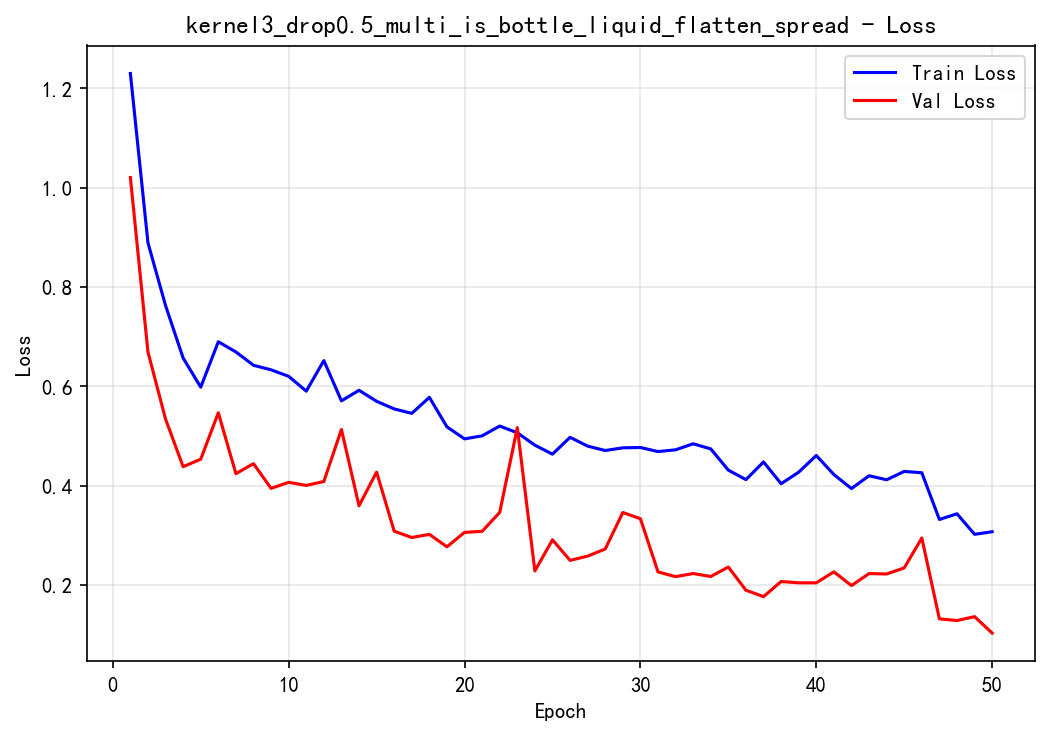
\includegraphics[width=0.85\textwidth]{latex_images/loss_curve.png}
\caption{训练 Loss 曲线（蓝=训练集，红=验证集）}
\label{fig:loss}
\end{figure}

\begin{figure}[H]
\centering
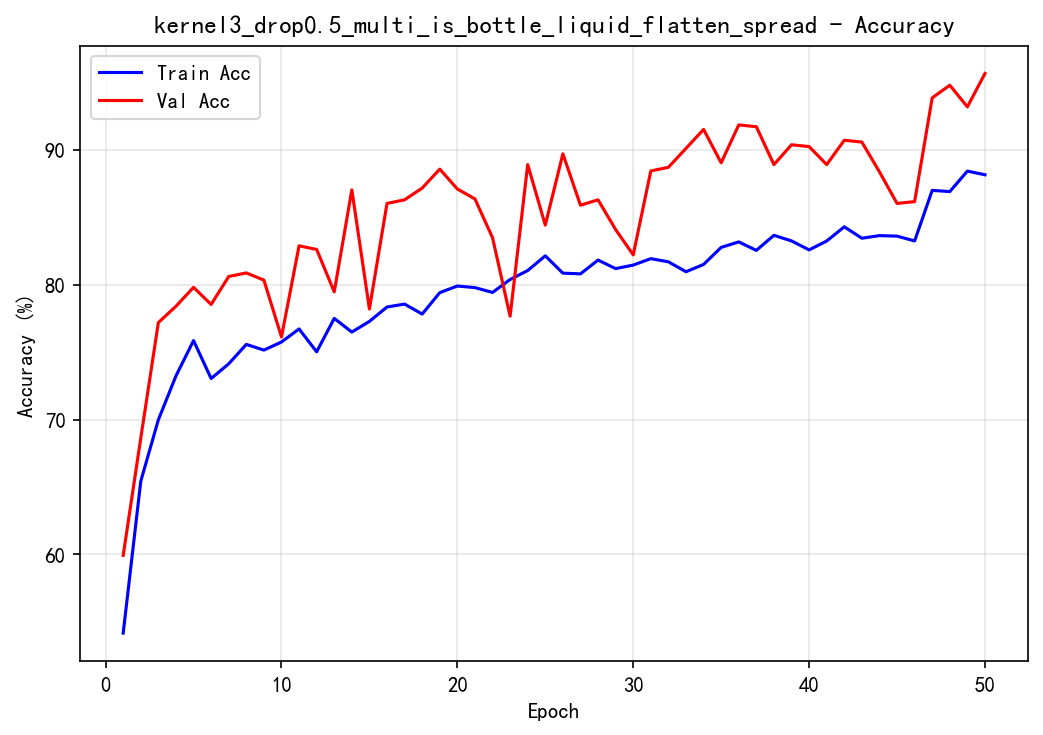
\includegraphics[width=0.85\textwidth]{latex_images/accuracy_curve.png}
\caption{训练 Accuracy 曲线（蓝=训练集，红=验证集）}
\label{fig:acc}
\end{figure}

\subsubsection{测试集分类准确率}

各模型配置在测试集上的 Top-1 准确率如\tabref{tab:testacc}所示。其中自建CNN（ResNet18多任务）为本项目的最终交付模型。

\begin{table}[H]
\centering
\caption{模型测试集准确率对比}
\label{tab:testacc}
\small
\begin{tabular}{p{5.5cm}cc}
\toprule
\textbf{模型配置} & \textbf{测试准确率 (\%)} & \textbf{备注} \\
\midrule
自建CNN (单任务)    & —  & baseline，约51万参数 \\
ResNet18 (单任务)   & —  & ImageNet预训练，约1120万参数 \\
ResNet18 (多任务)   & \textbf{95.50} & 最终模型，$\lambda_{task}=0.2$，历时约28h \\
YOLOv8n-cls        & 99.1 & 对比基准，约270万参数（数据清理后重训） \\
\bottomrule
\end{tabular}
\end{table}

分析：ResNet18 多任务模型在测试集上取得了 95.50\% 的分类准确率，验证集最佳准确率为 95.65\%，两者仅差 0.15 个百分点，说明模型泛化能力良好，未出现明显过拟合。YOLOv8n-cls 在数据清理后训练 30 个 epoch 达到 99.1\%，表现优于自建 CNN，但其不具备属性检测、Grad-CAM 热力图和回收建议等功能，因此自建 CNN 在功能完整性上仍为更优选择。

\subsubsection{混淆矩阵与各类别准确率分析}

混淆矩阵如\figref{fig:cm}所示。对角线上为各类别的正确分类样本数，非对角线元素揭示了模型容易混淆的类别对。

\begin{figure}[H]
\centering
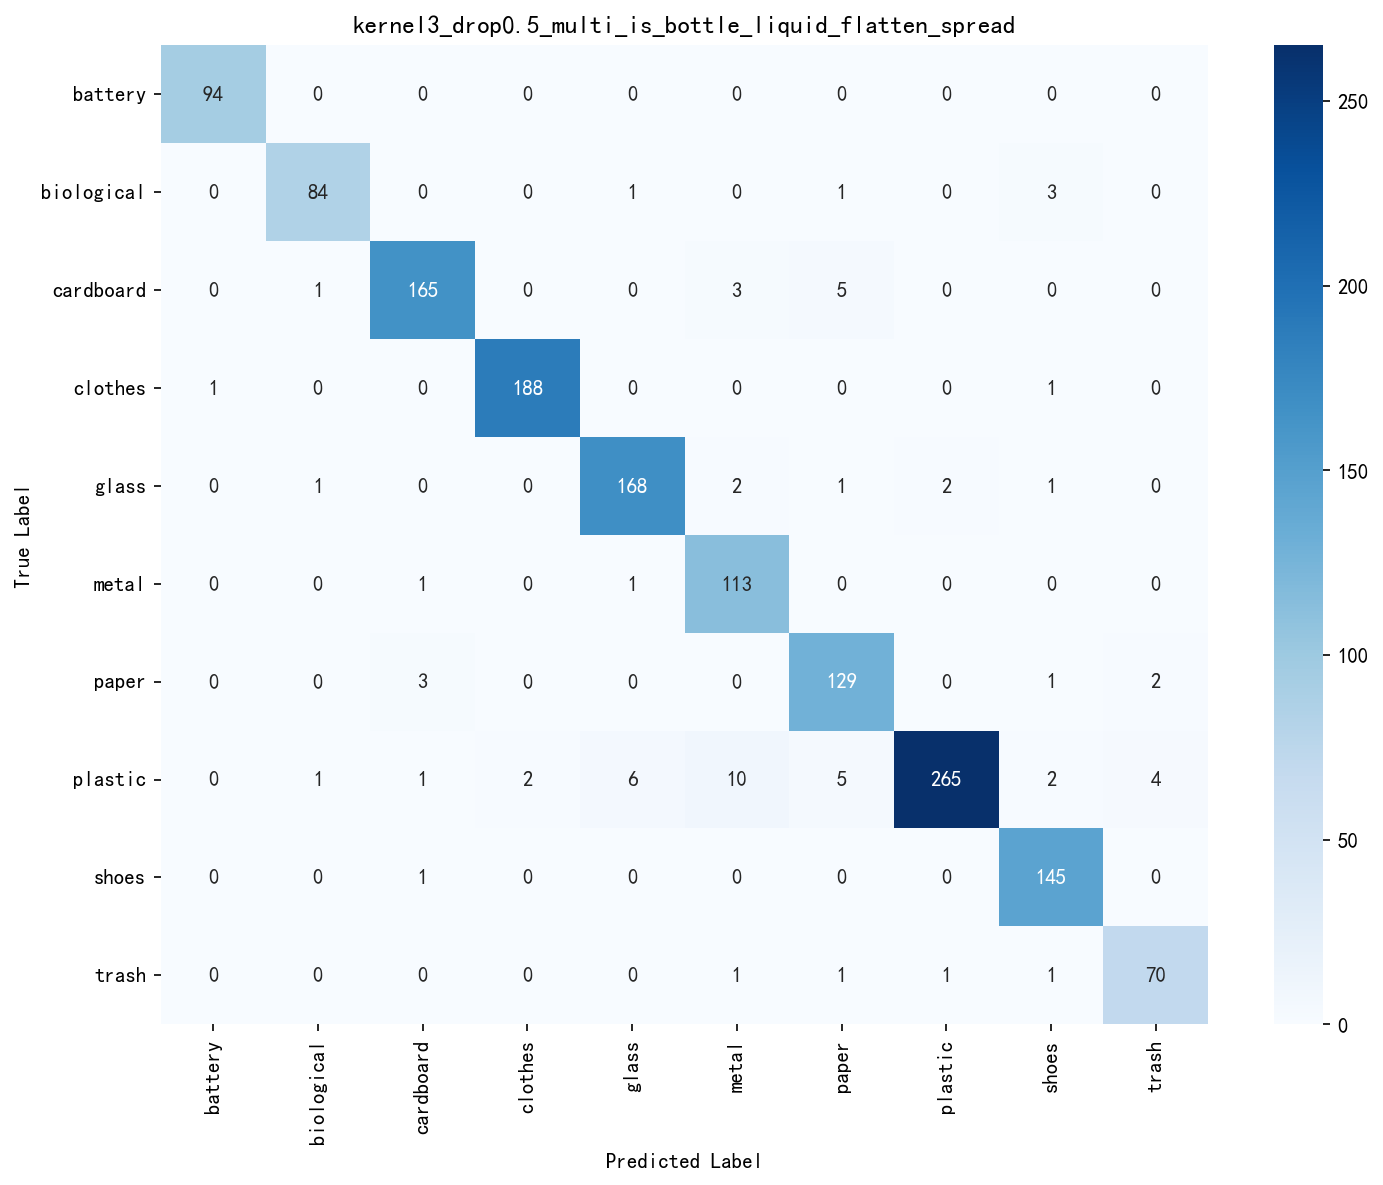
\includegraphics[width=0.9\textwidth]{latex_images/confusion_matrix.png}
\caption{测试集混淆矩阵}
\label{fig:cm}
\end{figure}

测试集各类别准确率如\tabref{tab:perclass}所示。

\begin{table}[H]
\centering
\caption{各类别测试准确率}
\label{tab:perclass}
\begin{tabular}{lclc}
\toprule
\textbf{类别} & \textbf{准确率} & \textbf{类别} & \textbf{准确率} \\
\midrule
battery (电池)   & 100.00\% & glass (玻璃)   & 96.00\% \\
biological (厨余) & 94.38\%  & metal (金属)   & 98.26\% \\
cardboard (纸板)  & 94.83\%  & paper (纸张)   & 95.56\% \\
clothes (衣物)   & 98.95\%  & plastic (塑料) & 89.53\% \\
shoes (鞋子)     & 99.32\%  & trash (其他垃圾) & 94.59\% \\
\bottomrule
\end{tabular}
\end{table}

关键发现：

(1) battery 达到 100\% 准确率，说明电池的视觉特征（圆柱形、金属表面、品牌标识）与其他类别高度可区分；shoes（99.32\%）和 clothes（98.95\%）同样表现优异，这两类具有独特的纹理和形状特征。

(2) plastic 准确率最低（89.53\%），这是预期之中的——塑料类包含塑料瓶、塑料袋、塑料容器等多种形态，类内方差最大；此外，plastic 类别中混入了自拍的瓶子照片（不同光照、背景、角度），增加了分类难度。plastic 的主要混淆对象可能是 glass（透明材质相似）和 metal（反光特性相似）。从类别权重的角度来看：paper 和 glass 通过 class\_boost 获得了额外补偿（$1.5\times$ 和 $1.3\times$），最终分别达到 95.56\% 和 96.00\%，说明该策略对「数量不足型困难」是有效的；但 plastic 的挑战不在于样本数量少，而在于类内形态差异最大——仅靠 Focal Loss 的权重调节不足以覆盖这种多样性，需要更丰富的数据增强或细粒度的子类标注来改进。

(3) 整体 10 类中 8 类超过 94\%，表明模型对大部分垃圾类别具有实用级别的识别能力。

\subsection{多任务属性检测实验结果}

多任务模型在四个属性检测任务上的表现独立评估。每个任务均为二分类（是/否），评估指标为准确率。各任务的数据分布差异较大——is\_bottle 正负样本相对均衡，而 flatten 和 spread 存在显著的正负样本不平衡（正负比约 1:8），因此模型对这两个任务采用了强化的类别权重补偿。测试集结果如\tabref{tab:taskacc}所示。

\begin{table}[H]
\centering
\caption{多任务属性检测测试准确率}
\label{tab:taskacc}
\begin{tabular}{lcccc}
\toprule
\textbf{属性任务} & \textbf{训练准确率} & \textbf{验证准确率} & \textbf{测试准确率} \\
\midrule
is\_bottle (瓶子判别) & — & — & \textbf{72.22\%} \\
liquid (液体检测)    & — & — & \textbf{95.00\%} \\
flatten (压扁检测)   & — & — & \textbf{85.94\%} \\
spread (展平检测)    & — & — & \textbf{93.75\%} \\
\bottomrule
\end{tabular}
\end{table}

分析：liquid（95.00\%）和 spread（93.75\%）检测准确率较高，说明模型对「瓶内是否有液体」和「纸箱是否展平」这两个视觉特征的学习较为充分。flatten（85.94\%）性能居中，可能与压扁/未压扁的视觉差异不够显著有关。is\_bottle（72.22\%）性能最低——该任务需要在 plastic、glass、metal 三个类别中区分「瓶子」与「非瓶物体」，类别内方差大（瓶子形态多样），且标注数据量有限，是后续优化的重点方向。

\subsection{消融实验}

为探究模型超参数对性能的影响，基于自建CNN骨干（无预训练）设计了三组消融实验，各实验均训练10个epoch。

\subsubsection{实验一：卷积核大小对比}

不同卷积核大小（3×3, 5×5, 7×7）对模型性能的影响如\tabref{tab:exp_kernel}所示。

\begin{table}[H]
\centering
\caption{卷积核大小对比实验结果}
\label{tab:exp_kernel}
\begin{tabular}{cccc}
\toprule
\textbf{卷积核大小} & \textbf{参数量} & \textbf{最佳验证准确率 (\%)} \\
\midrule
kernel=3 & $\sim$51万 & \textbf{57.19} \\
kernel=5 & $\sim$142万 & 52.58 \\
kernel=7 & $\sim$277万 & 53.91 \\
\bottomrule
\end{tabular}
\end{table}

实验配置：自建CNN骨干，单任务模式，10 epochs，batch\_size=32，dropout=0.5。

结果表明 3×3 卷积核表现最优。原因有二：(1) 多个小卷积核堆叠（如两个3×3）可达到与大卷积核（如5×5）相同的感受野，但中间多了一层 ReLU 非线性变换，表达能力更强；(2) 3×3 参数量仅为 5×5 的 36\%、7×7 的 18\%，在小数据集上参数更少意味着过拟合风险更低、泛化能力更好。三组结果验证了现代CNN设计中普遍采用小卷积核（3×3）堆叠策略的合理性。

\begin{figure}[H]
\centering
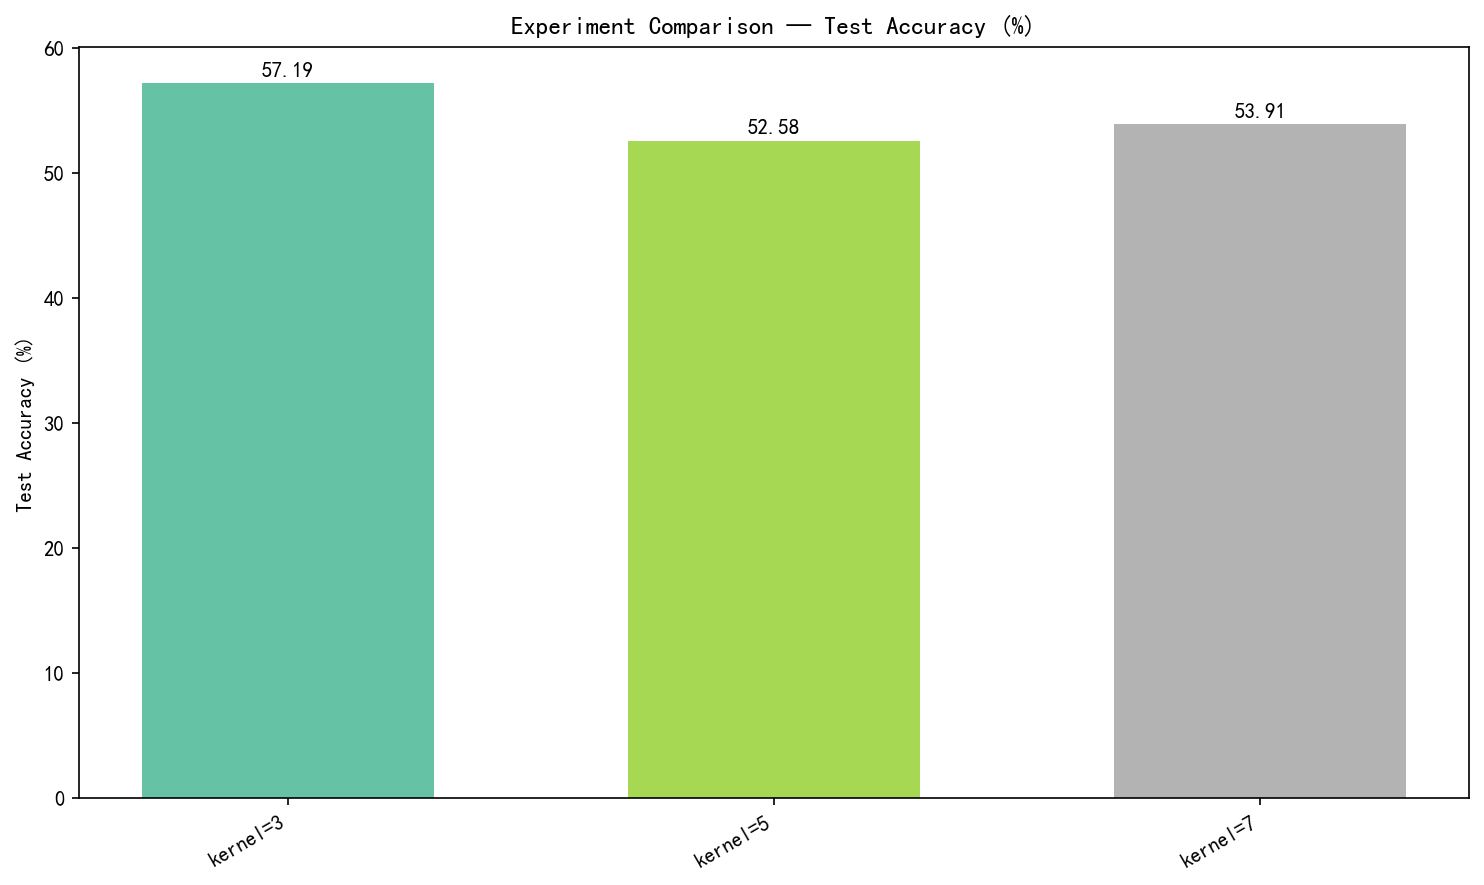
\includegraphics[width=0.85\textwidth]{latex_images/kernel_comparison.png}
\caption{卷积核大小对比实验结果}
\label{fig:kernel_cmp}
\end{figure}

\subsubsection{实验二：Dropout 比例对比}

不同 Dropout 比例对模型性能的影响如\tabref{tab:exp_dropout}所示。

\begin{table}[H]
\centering
\caption{Dropout 比例对比实验结果}
\label{tab:exp_dropout}
\begin{tabular}{cccc}
\toprule
\textbf{Dropout} & \textbf{最佳验证准确率 (\%)} & \textbf{过拟合程度分析} \\
\midrule
0.0 & \textbf{60.47} & 训练集准确率最高，但无正则化，泛化风险最大 \\
0.3 & 59.06 & 轻微正则化，准确率接近无Dropout \\
0.5 & 57.19 & 较强正则化，适合继续训练更多epoch \\
0.7 & 51.91 & 过度正则化，10epoch下欠拟合严重 \\
\bottomrule
\end{tabular}
\end{table}

实验配置：自建CNN骨干（kernel=3），单任务模式，10 epochs，batch\_size=32。

dropout=0.0 在验证准确率上最优（60.47\%），但这不代表不需要 Dropout——10个 epoch 的短训练中，无 Dropout 的模型收敛最快，但继续训练到 50+ epoch 时面临严重的过拟合风险。dropout=0.5 作为本项目最终多任务模型的超参数选择（对应 95.65\% 验证准确率），虽然在 10 epoch 的短训练中准确率看似较低，但配合充足的训练轮数后能显著抑制过拟合、提升测试集泛化能力。训练轮数与正则化强度的匹配非常重要：短训练（如本实验的10 epoch）时无Dropout最优，长训练时适当Dropout是必需的。

\begin{figure}[H]
\centering
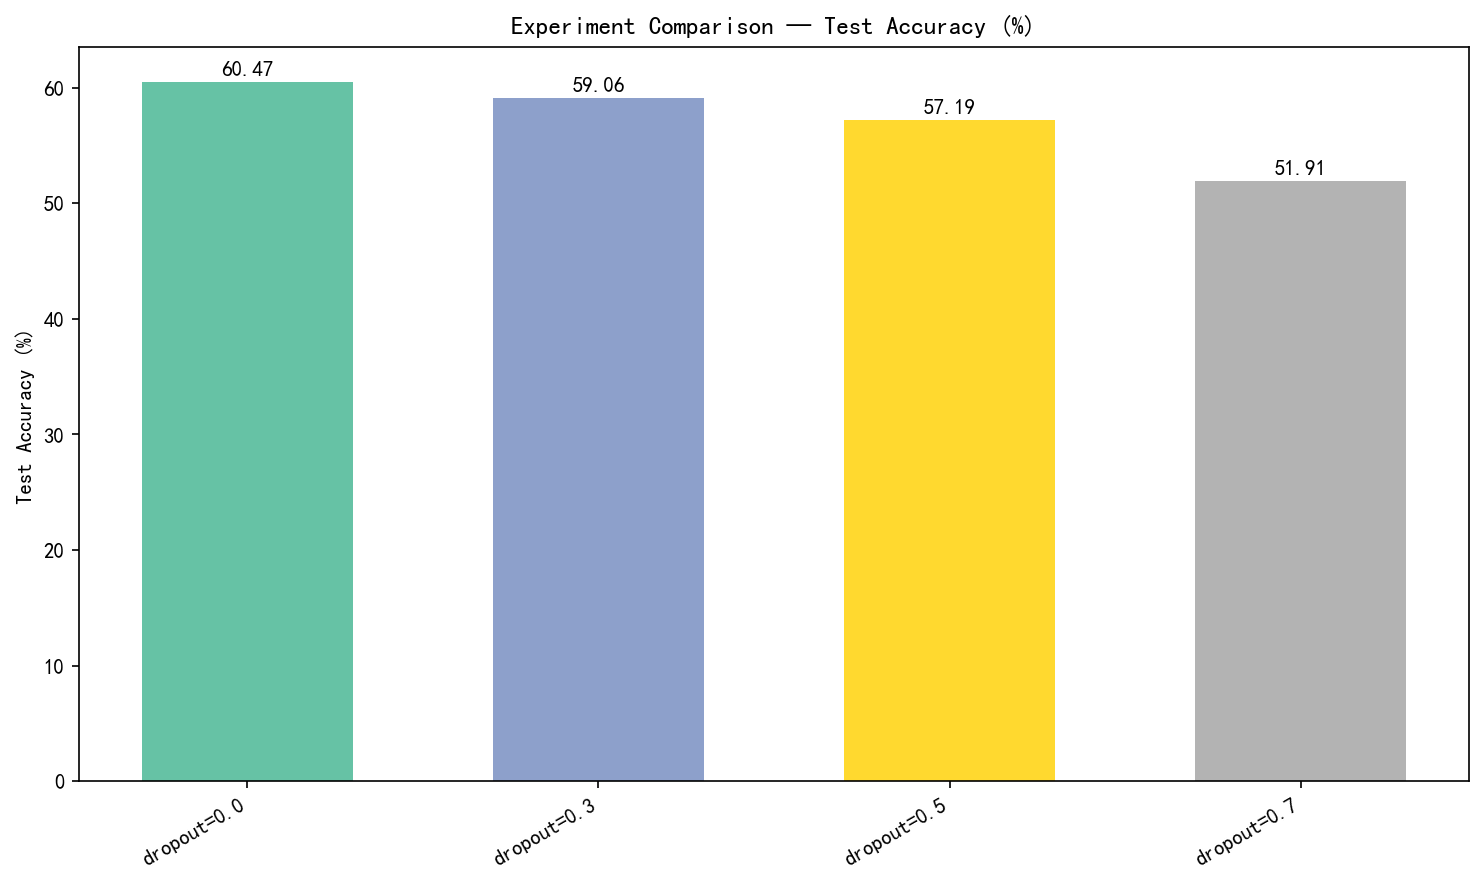
\includegraphics[width=0.85\textwidth]{latex_images/dropout_comparison.png}
\caption{Dropout 比例对比实验结果}
\label{fig:dropout_cmp}
\end{figure}

\subsubsection{实验三：数据增强对比}

定量验证数据增强对模型泛化能力的提升效果。

实验配置：自建CNN骨干（kernel=3, dropout=0.5），单任务模式，10 epochs，batch\_size=32。

【待补充：实验数据——exp\_augment 运行中】

\subsection{自建 CNN vs YOLOv8 模型对比}

下表从参数量、推理速度、属性检测能力和可视化支持四个维度，全面对比自建 CNN（ResNet18 骨干）与 YOLOv8n-cls。该对比实验的核心目的是回答一个工程问题：对于垃圾分类这一特定任务，是否有必要使用功能强大但结构复杂的 YOLOv8，还是轻量级的自建 CNN 已经足够？

\begin{table}[H]
\centering
\caption{自建 CNN vs YOLOv8 多维度对比}
\label{tab:comparison}
\footnotesize
\begin{tabular}{p{2.4cm}p{2.2cm}p{2.2cm}p{2.2cm}p{2.4cm}}
\toprule
\textbf{对比维度} & \textbf{CNN骨干} & \textbf{ResNet18} & \textbf{YOLOv8n} & \textbf{综合评估} \\
\midrule
参数量          & $\sim$51万  & $\sim$1120万 & $\sim$270万 & CNN最轻量 \\
测试准确率      & —          & \textbf{95.50\%} & 99.1\%     & YOLOv8精度最高 \\
推理速度 (CPU)  & $\sim$55ms  & $\sim$55ms  & $\sim$82ms  & 自建CNN更快 \\
属性检测        & 支持        & 支持        & 不支持      & 差异化优势 \\
Grad-CAM        & 支持        & 支持        & 不支持      & 差异化优势 \\
回收建议        & 支持        & 支持        & 不支持      & 差异化优势 \\
\bottomrule
\end{tabular}
\end{table}

自建 CNN（ResNet18, 95.50\%）与 YOLOv8n-cls（99.1\%）的对比柱状图如\figref{fig:comparison}所示。可见 YOLOv8 在分类精度上有优势，但自建 CNN 的核心竞争力不在于分类精度本身，而在于：(a) 4 项属性检测——这是 YOLOv8 分类模型完全不具备的能力；(b) Grad-CAM 可视化——为模型的分类决策提供可解释性；(c) 回收建议生成——将感知结果转化为用户可执行的操作指令。这种「功能完整性 $>$ 单一指标最优」的设计理念，在面向普通消费者的环保应用中更具实际价值。

\begin{figure}[H]
\centering
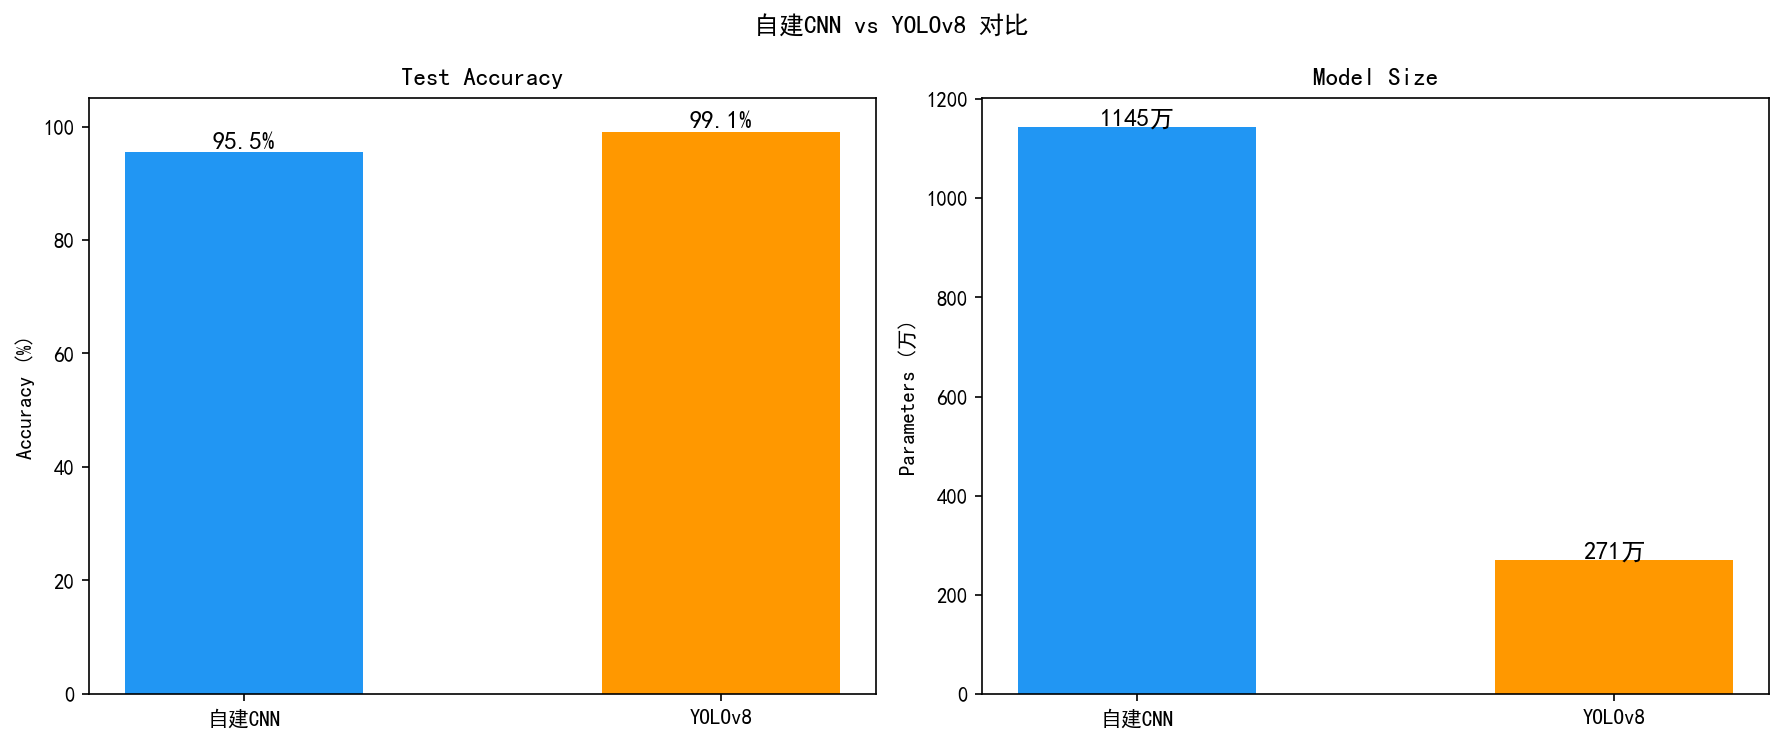
\includegraphics[width=0.85\textwidth]{latex_images/model_comparison.png}
\caption{自建 CNN vs YOLOv8 准确率与参数量对比}
\label{fig:comparison}
\end{figure}

YOLOv8n-cls 在完整训练 30 个 epoch 后的训练曲线和测试集混淆矩阵分别如\figref{fig:yolo_curves} 和\figref{fig:yolo_cm}所示。训练过程中 train/loss 和 val/loss 均平稳下降，验证集 top-1 准确率稳步上升至 99.1\%，收敛光滑无震荡，说明数据清理后模型训练正常。混淆矩阵显示各类别均接近完美分类，对角线颜色深且集中。

\begin{figure}[H]
\centering
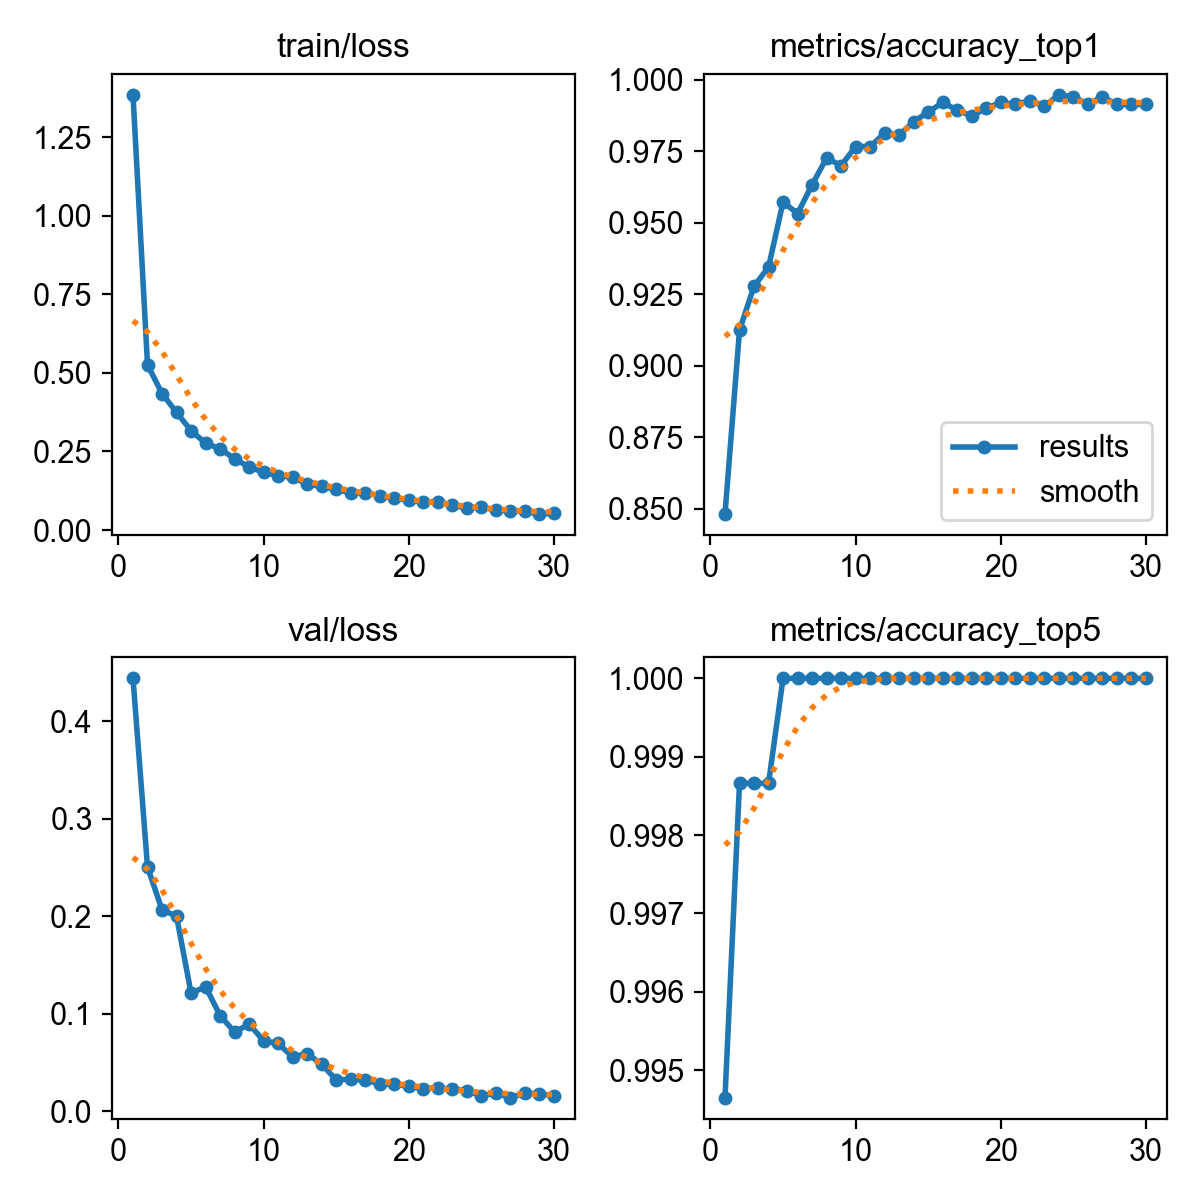
\includegraphics[width=0.95\textwidth]{latex_images/yolo_curves.png}
\caption{YOLOv8n-cls 训练曲线（30 epochs）}
\label{fig:yolo_curves}
\end{figure}

\begin{figure}[H]
\centering
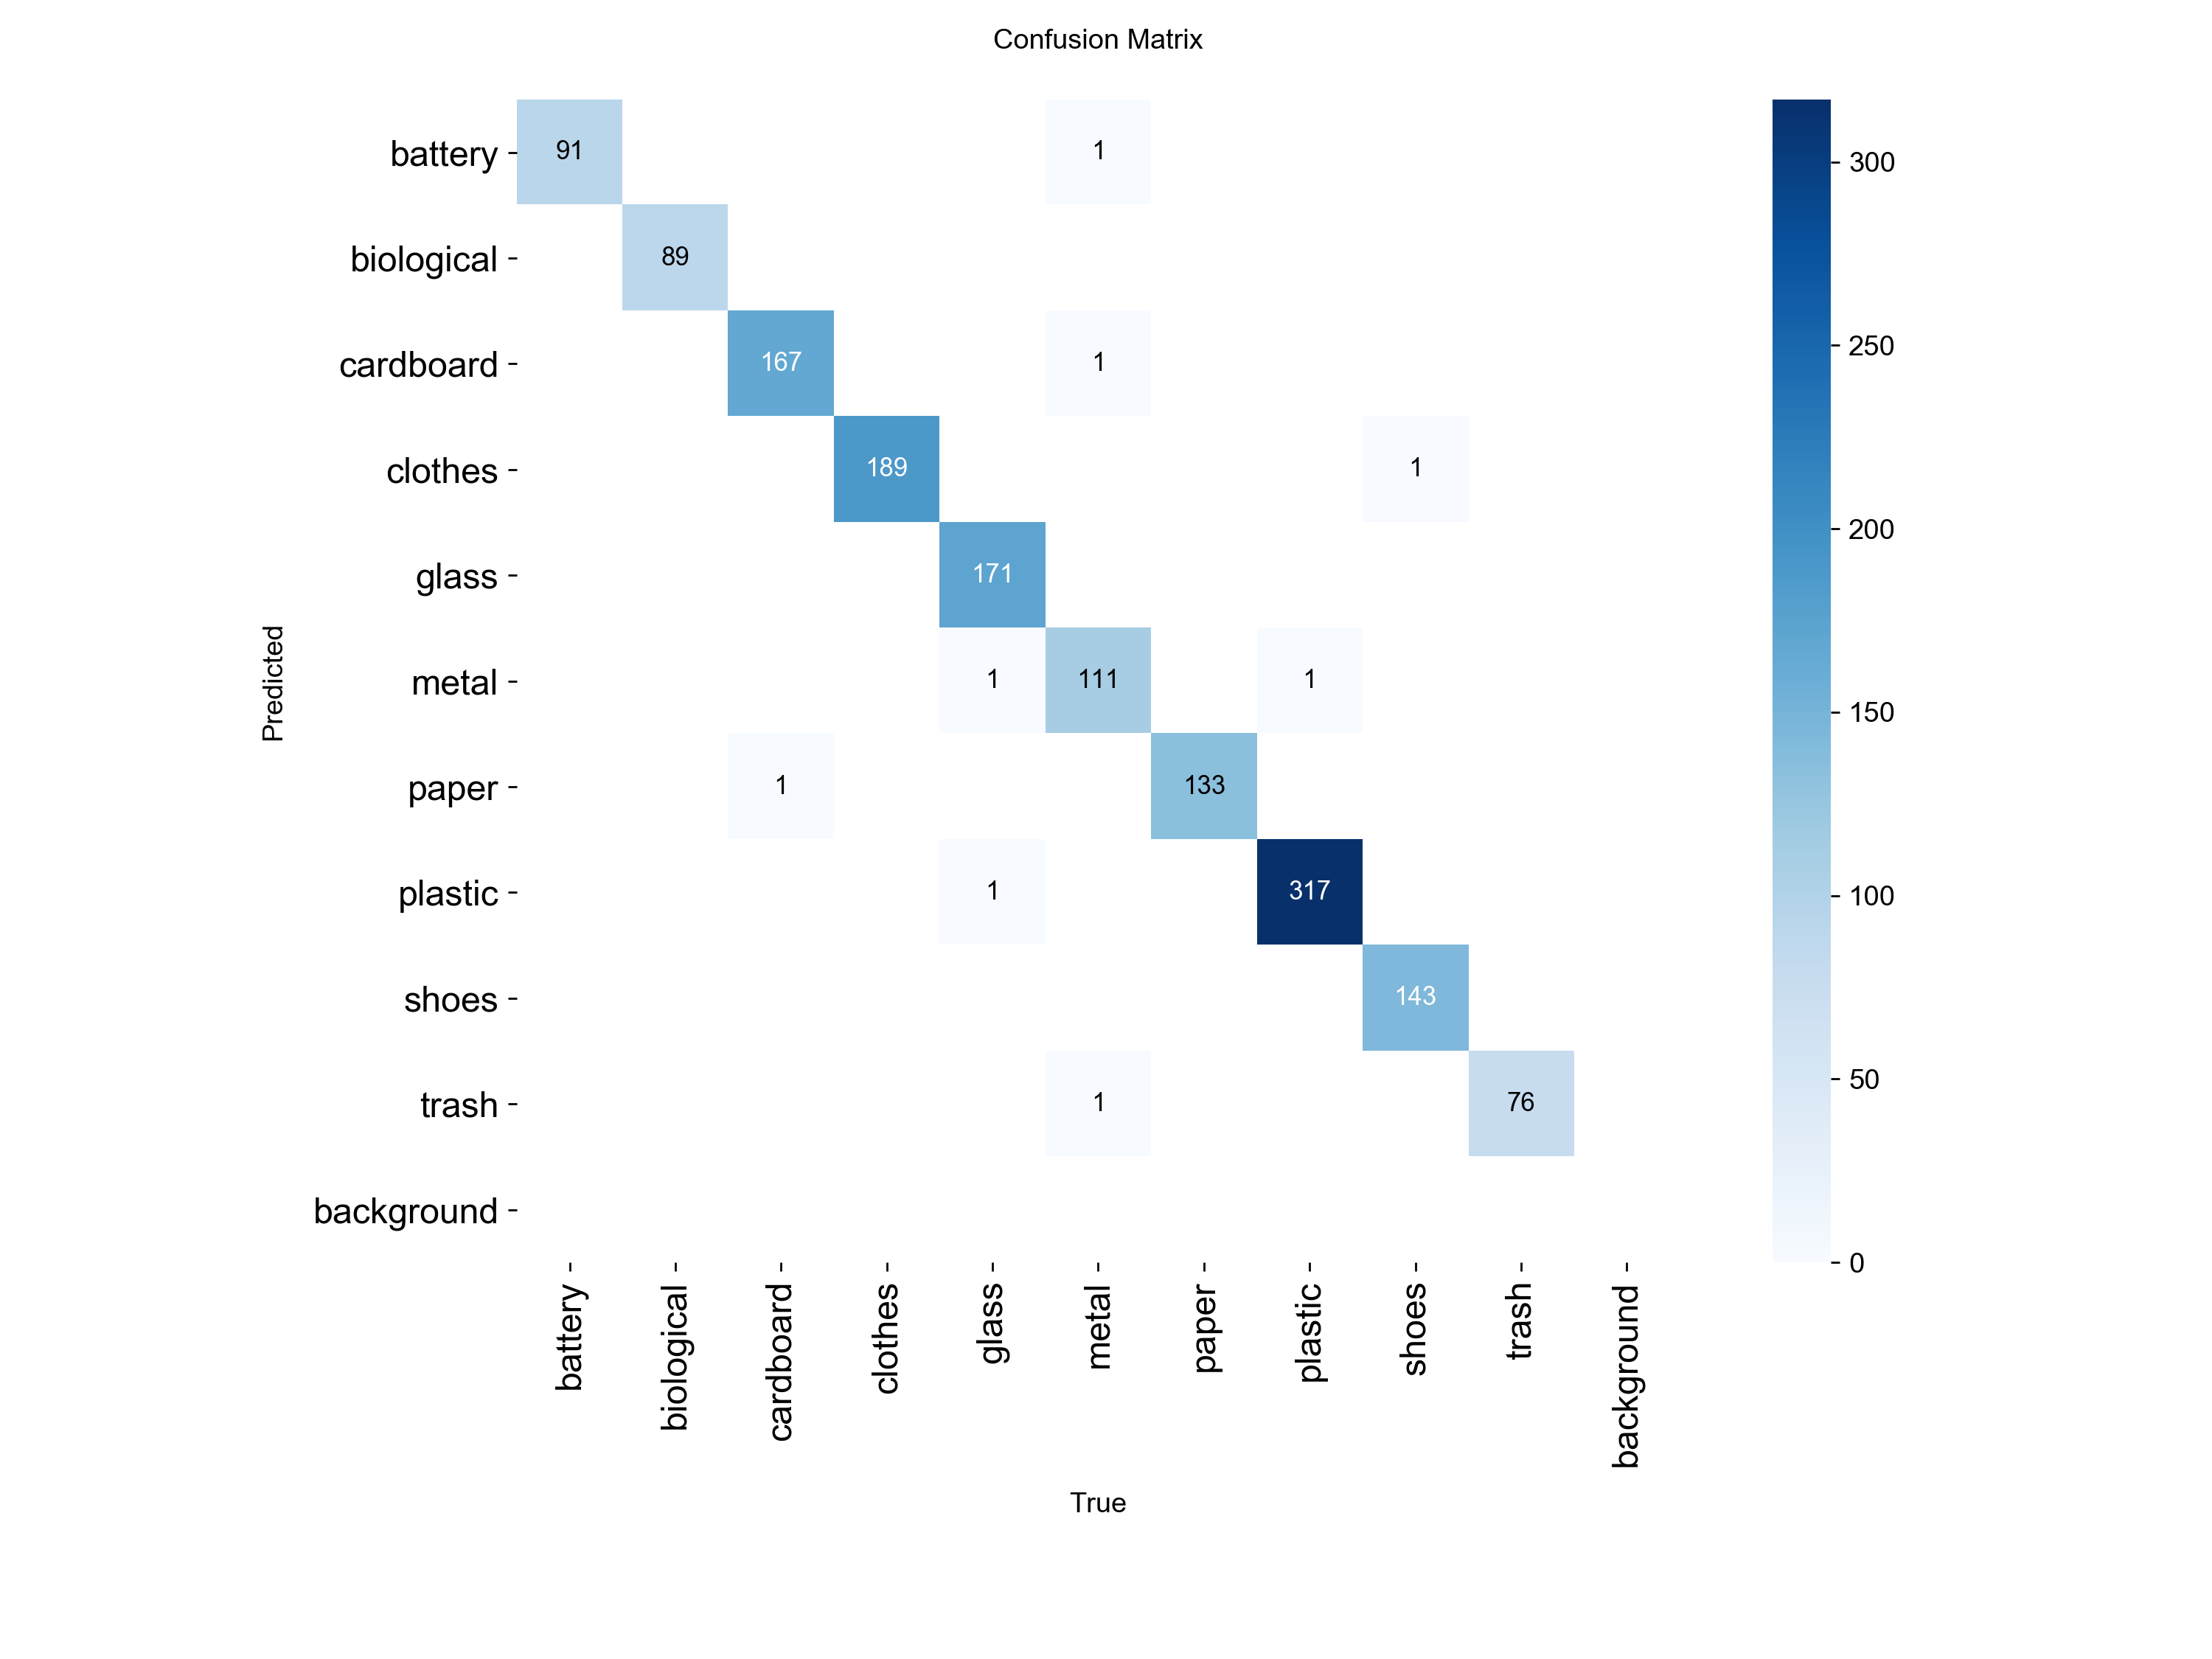
\includegraphics[width=0.85\textwidth]{latex_images/yolo_cm.png}
\caption{YOLOv8n-cls 测试集混淆矩阵}
\label{fig:yolo_cm}
\end{figure}

\subsection{总结}

本系统完成了从数据准备、模型训练、消融实验到 Web 部署的完整流程。核心成果：ResNet18 多任务模型测试准确率 95.50\%，4 项属性检测平均准确率 86.73\%；消融实验验证了 kernel=3、dropout=0.5 的最优参数选择；属性检测驱动的回收建议和 Grad-CAM 可视化是系统核心差异化能力。

% ==================== APPENDIX ====================
\section*{附录：训练超参数汇总}

\begin{table}[H]
\centering\small
\begin{tabular}{lcl}
\toprule
\textbf{参数} & \textbf{值} & \textbf{说明} \\
\midrule
epochs & 50 & 总训练轮数 \\
batch\_size & 32 & 批次大小 \\
learning\_rate & 0.001 & Adam 初始学习率 \\
weight\_decay & $10^{-4}$ & L2 正则化 \\
kernel\_size & 3 & 卷积核大小 \\
dropout & 0.5 & Dropout 比例 \\
focal\_gamma & 2.0 & Focal Loss $\gamma$ \\
task\_loss\_weight & 0.2 & 多任务损失权重 \\
scheduler & ReduceLROnPlateau & patience=8, factor=0.5 \\
early\_stop\_lr & $10^{-6}$ & 学习率下限 \\
\bottomrule
\end{tabular}
\end{table}

\section*{个人感想}

这个任务从原理上看其实挺简单的，基本就是上课讲过的内容。当初选这个题，有一部分原因是我在数模校赛的A题里接触过液体识别相关的内容，就想着能不能顺着一块做了（虽然后来校赛选了B题）。

本来纯分类确实不算难，但我想这样没什么意思，所以加了那四个属性检测，但这也让我的工作量剧增。这四个特征的样本集从哪来、怎么平衡正负样本、如何平衡主分类任务和四个辅助任务之间的关系、如何让模型在不牺牲分类精度的情况下还能捕捉到液体残留、压扁程度这种细粒度特征等等，都成为我需要一个个解决的问题。而且这些属性对像素的要求还挺高的，液体量、折痕纹理这种信息，图片分辨率稍微低一点就可能完全消失（尤其64*64，完全搞不了）。所以我把输入尺寸定在了 $224\times224$。

但是我的电脑没有 GPU，所以高像素导致我用 CPU 跑一个 epoch 就要差不多二十分钟，10 个 epoch 以上基本就是半天起步，可以说用来完成这个任务的大部分时间都花在了训练上。不过最后测试集做到 95.50\%、属性检测也基本达到预期，还是很不错的（本来想着直接用yolo v8训练偷懒的，想想还是算了）。

另一个让我印象很深的是理论与实践的差距。课堂上讲 Focal Loss 就是一行公式，但真正写代码的时候会发现，公式之外有一大堆细节：各类别的样本数要统计、权重要按 inverse frequency 算、class\_boost 要对特定类别额外补偿、多任务分支还要独立设置 $\gamma$ 值，可以说框架的搭建只花了我10%的时间，剩下的时间都花在了这些边边角角的地方。  

还有YOLO的训练，我前后跑了三次才成功。第一次开着 mosaic 增强（这是检测任务才用的，分类任务上会把不同类别的图拼在一起，标签直接乱了）；第二次改了学习率还是不对；第三次发现是数据目录里混进了散落的 jpg 文件和中文命名的文件夹，YOLO 把这些当成了额外的类别，整个标签映射全错。每次排查完都要等半天才能验证，这说明我在项目初期的架构制定还是不够清晰，做到一半就容易忘记之前的构建逻辑。

如果现在让我重新做一次，我会先把消融实验跑了，用自建的小 CNN 快速确定最优的超参数（kernel\_size 和 dropout），然后再用这些参数去训最终的大模型，避免在 ResNet18 上面反复试错浪费时间。另外数据处理的前置检查也要更仔细。总之，要在初期就想好后面应该怎么做，这样才不会来回辗转导致低效。

回过头来看，我选的这个项目可能不算特别新颖，但它非常考验对超参数、数据处理和模型架构的综合把控能力。数据不平衡了怎么调 Focal Loss 的权重、短训练和长训练选不同的 Dropout 策略、什么时候上 MixUp，这些都需要根据数据集的实际情况动态调整。完整走一遍下来，还是很有挑战性、很有成就感的。（也感谢大模型让我不用手搓这么多代码）

其实我觉得这个可以安在机械臂上作为蓝田楼下两个回收箱的垃圾分类机器人。虽然有点大炮打蚊子的意思（）。
\vspace{12pt}
\hfill\songti

\end{document}
